\documentclass[12pt,a4paper]{article}
\usepackage[spanish]{babel}
\usepackage[utf8]{inputenc}
\usepackage[T1]{fontenc}
\usepackage[letterpaper,top=2cm,bottom=5cm,left=3cm,right=3cm]{geometry}
\usepackage{graphicx,booktabs,array,xcolor,amsmath,hyperref}
\usepackage{titlesec,fancyhdr,parskip,enumitem,tcolorbox}
\usepackage{caption,float,subcaption,microtype,longtable}
\tcbuselibrary{skins,breakable}
\newtcolorbox{cajainfo}[1]{colback=black!5,colframe=black,
  fonttitle=\bfseries\small,title=#1,breakable,left=6pt,right=6pt}
\pagestyle{fancy}\fancyhf{}
\setlength{\headheight}{70pt}\renewcommand{\headrulewidth}{0.4pt}
\fancyhead[C]{%
  \begin{minipage}[c]{2.5cm}\centering
    
\includegraphics[width=2.2cm]{imagenes/uta.png}
  \end{minipage}\hfill
  \begin{minipage}[c]{8cm}\centering
    \small{\textbf{UNIVERSIDAD T\'ECNICA DE AMBATO}}\\[0.1cm]
    \scriptsize\textit{FACULTAD DE INGENIER\'IA EN SISTEMAS ELECTR\'ONICA E INDUSTRIAL}\\[0.1cm]
    \scriptsize\textbf{CARRERA DE SOFTWARE}\\[0.1cm]
    \scriptsize\textbf{CICLO ACAD\'EMICO: FEBRERO -- JULIO 2026}
  \end{minipage}
  \hfill\begin{minipage}[c]{2.5cm}\centering
    
\includegraphics[width=2.2cm]{imagenes/fisei.png}
  \end{minipage}
}
\fancyfoot[C]{\thepage}
\titleformat{\section}{\large\bfseries}{\thesection}{1em}{}[\titlerule]
\titleformat{\subsection}{\normalsize\bfseries}{\thesubsection}{1em}{}
\begin{document}
\begin{center}{\large\textbf{INFORME DE GU\'IA PR\'ACTICA}}\end{center}
\section{Portada}
\begin{flushleft}\renewcommand{\arraystretch}{1.3}
\begin{tabular}{@{} l p{10cm} @{}}
  \textbf{Tema:} & An\'alisis Exploratorio de Datos para Machine Learning \\
  \textbf{Dataset:} & \texttt{alquileres\_etiquetados.csv} \\
  \textbf{Unidad de Organizaci\'on Curricular:} & Profesional. \\
  \textbf{Nivel y Paralelo:} & 6to -- A \\
  \textbf{Alumnos:} & Toala Camacho Steeven Santiago. \\ & Alexis Eduardo Lopez Guerrero. \\
  \textbf{Asignatura:} & Inteligencia de Negocios \\
  \textbf{Docente:} & Ing. Rub\'en Nogales. \\
\end{tabular}\end{flushleft}
\section{Objetivos}
\subsection*{Objetivo General}
Realizar un an\'alisis exploratorio del dataset de alquileres de pel\'iculas
para identificar patrones, distribuciones y relaciones entre variables
que orienten la preparaci\'on de datos para modelos de Machine Learning.
\subsection*{Objetivos Espec\'ificos}
\begin{enumerate}[label=\arabic*.]
  \item Visualizar la relaci\'on entre variables num\'ericas mediante scatter plots.
  \item Calcular e interpretar la matriz de covarianza y correlaci\'on.
  \item Analizar la distribuci\'on acumulada (ECDF) de cada feature.
  \item Comparar los features seg\'un las etiquetas de clasificaci\'on.
\end{enumerate}
\section{Introducci\'on}
El an\'alisis exploratorio de datos (EDA) es una etapa fundamental en cualquier
proyecto de Machine Learning. Permite entender la distribuci\'on de los datos,
detectar valores at\'ipicos, identificar correlaciones y validar supuestos
antes de entrenar un modelo.

\begin{cajainfo}{Dataset: alquileres\_etiquetados.csv}
El dataset contiene \textbf{16044 registros} y \textbf{11 variables}. 
Los features num\'ericos analizados son: \texttt{ingreso},
\texttt{veces\_alquilada\_pelicula} y \texttt{precio\_promedio\_genero}.
Las etiquetas binarias son: \texttt{ingreso\_alto}, \texttt{pelicula\_popular}
y \texttt{genero\_alto\_valor}.
\end{cajainfo}
\section{Estad\'isticas Descriptivas}
\begin{table}[H]\centering
  \caption{Estad\'isticas descriptivas de los features num\'ericos}
  \begin{tabular}{lccc}\toprule
    \textbf{Estad\'istico} & \textbf{Ingreso} & \textbf{Veces alquilada} & \textbf{Precio prom.}\\\midrule
    count & 16044.000 & 16044.000 & 16044.000 \\
    mean & 4.201 & 19.406 & 4.203 \\
    std & 2.363 & 6.394 & 0.262 \\
    min & 0.000 & 4.000 & 3.860 \\
    25% & 2.990 & 15.000 & 3.940 \\
    50% & 3.990 & 20.000 & 4.130 \\
    75% & 4.990 & 24.000 & 4.420 \\
    max & 11.990 & 34.000 & 4.660 \\
  \bottomrule\end{tabular}
\end{table}
\section{Scatter Plot}
El scatter plot permite visualizar la relaci\'on entre dos variables
y observar c\'omo se separan las clases en el espacio de features.
\begin{figure}[H]\centering
  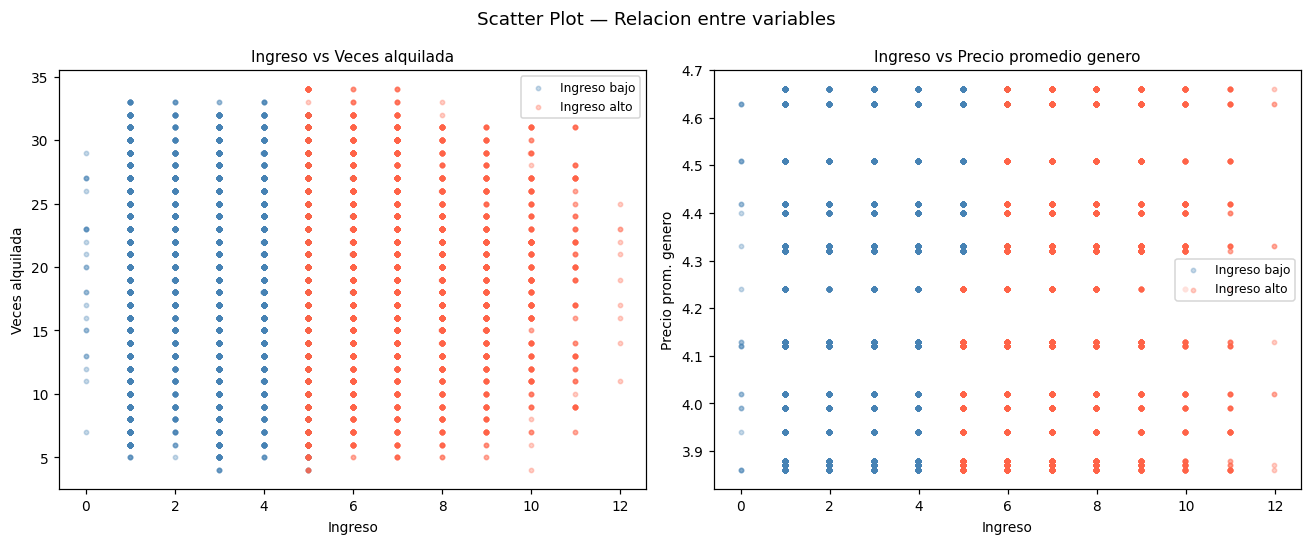
\includegraphics[width=0.95\textwidth]{imagenes_eda/scatter.png}
  \caption{Scatter Plot — Variables num\'ericas coloreadas por etiqueta \texttt{ingreso\_alto}}
\end{figure}
\begin{itemize}
  \item Los puntos \textbf{azules} representan registros con ingreso bajo (clase~0).
  \item Los puntos \textbf{rojos} representan registros con ingreso alto (clase~1).
  \item Se observa si existe separabilidad visual entre clases.
\end{itemize}
\section{Matriz de Covarianza}
La covarianza mide cu\'anto se mueven juntas dos variables en sus unidades originales.
Un valor positivo indica que suben juntas; negativo, que se mueven en sentido contrario.
\begin{figure}[H]\centering
  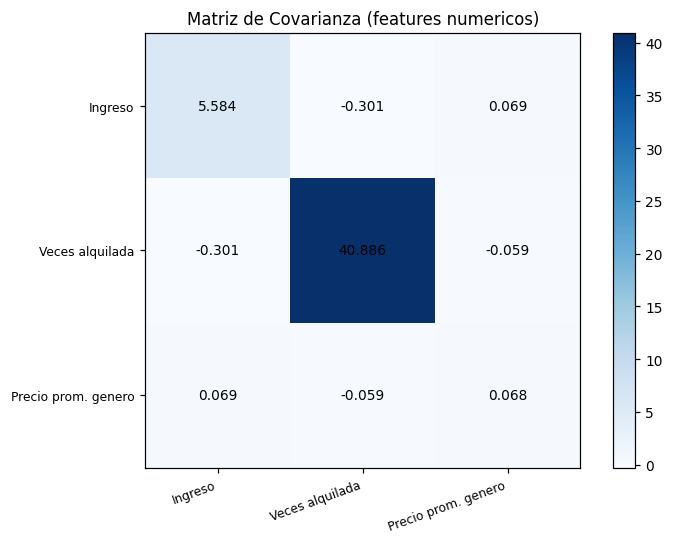
\includegraphics[width=0.7\textwidth]{imagenes_eda/covarianza.png}
  \caption{Matriz de Covarianza de los features num\'ericos}
\end{figure}
\begin{table}[H]\centering
  \caption{Valores de la matriz de covarianza}
  \begin{tabular}{lccc}\toprule
    \textbf{Feature} & \textbf{Ingreso} & \textbf{Veces alquilada} & \textbf{Precio prom. genero}\\\midrule
    Ingreso & 5.584 & -0.301 & 0.069 \\
    Veces alquilada & -0.301 & 40.886 & -0.059 \\
    Precio prom. genero & 0.069 & -0.059 & 0.068 \\
  \bottomrule\end{tabular}
\end{table}
\begin{itemize}
  \item La diagonal contiene la varianza de cada variable.
  \item La mayor covarianza fuera de la diagonal es entre \textbf{Ingreso} y \textbf{Veces alquilada} (-0.301).
\end{itemize}
\section{Matriz de Correlaci\'on}
La correlaci\'on normaliza la covarianza al rango $[-1, +1]$, lo que
permite comparar la fuerza de relaci\'on entre variables.
\begin{figure}[H]\centering
  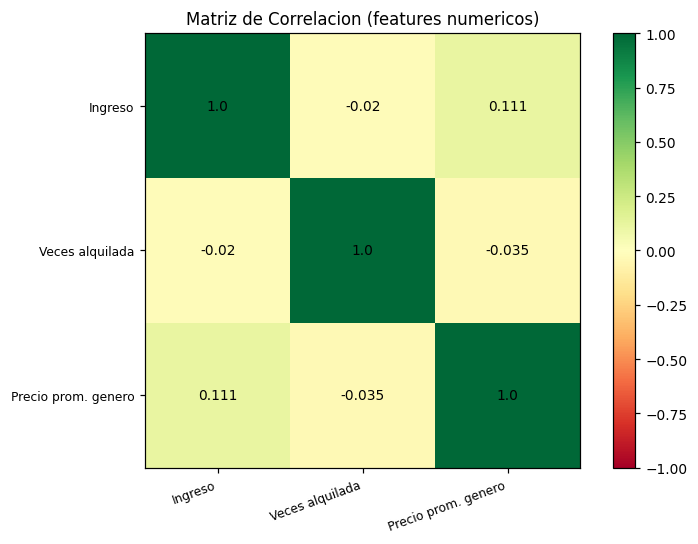
\includegraphics[width=0.7\textwidth]{imagenes_eda/correlacion.png}
  \caption{Matriz de Correlaci\'on de los features num\'ericos}
\end{figure}
\begin{table}[H]\centering
  \caption{Valores de la matriz de correlaci\'on}
  \begin{tabular}{lccc}\toprule
    \textbf{Feature} & \textbf{Ingreso} & \textbf{Veces alquilada} & \textbf{Precio prom. genero}\\\midrule
    Ingreso & 1.000 & -0.020 & 0.111 \\
    Veces alquilada & -0.020 & 1.000 & -0.035 \\
    Precio prom. genero & 0.111 & -0.035 & 1.000 \\
  \bottomrule\end{tabular}
\end{table}
\begin{itemize}
  \item Valores cercanos a $\pm 1$ indican alta correlaci\'on lineal.
  \item Valores cercanos a $0$ indican poca o ninguna relaci\'on lineal.
  \item Correlaciones altas entre features (multicolinealidad) pueden
        afectar negativamente a ciertos modelos de ML.
\end{itemize}
\section{Estad\'istica Acumulativa (ECDF)}
La ECDF muestra la proporci\'on del dataset con valor menor o igual a $x$.
Sirve para detectar outliers, ver distribuciones y rangos sin elegir bins.
\begin{figure}[H]\centering
  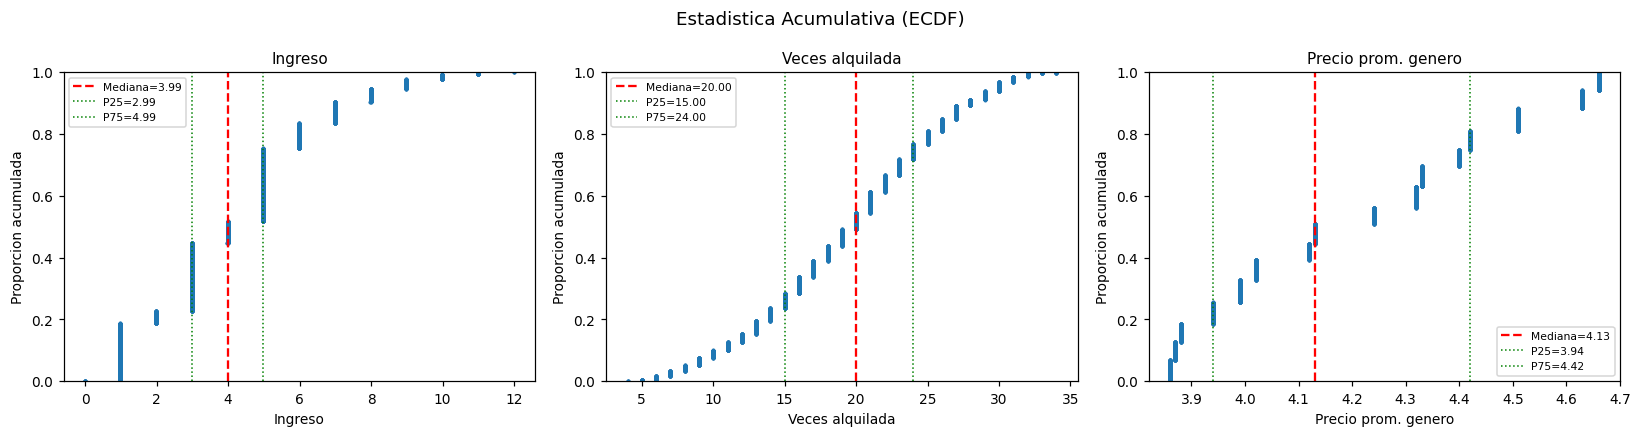
\includegraphics[width=0.95\textwidth]{imagenes_eda/ecdf.png}
  \caption{ECDF de los tres features num\'ericos}
\end{figure}
\begin{table}[H]\centering
  \caption{Estad\'isticos clave por feature (ECDF)}
  \begin{tabular}{lcccccc}\toprule
    \textbf{Feature} & \textbf{Media} & \textbf{Std} & \textbf{Min} & \textbf{P25} & \textbf{P50} & \textbf{Max}\\\midrule
    Ingreso & 4.201 & 2.363 & 0.000 & 2.990 & 3.990 & 11.990 \\
    Veces alquilada & 19.406 & 6.394 & 4.000 & 15.000 & 20.000 & 34.000 \\
    Precio prom. genero & 4.203 & 0.262 & 3.860 & 3.940 & 4.130 & 4.660 \\
  \bottomrule\end{tabular}
\end{table}
\section{An\'alisis por Etiqueta de Clasificaci\'on}
Se comparan los promedios de cada feature seg\'un el valor de cada etiqueta binaria.
\subsection{Ingreso Alto}
\begin{table}[H]\centering
  \caption{Media de features por clase -- Ingreso Alto}
  \begin{tabular}{lccc}\toprule
    \textbf{Clase} & \textbf{Ingreso} & \textbf{Veces alquilada} & \textbf{Precio prom.}\\\midrule
    Clase 0 & 2.796 & 19.473 & 4.226 \\
    Clase 1 & 6.584 & 19.293 & 4.164 \\
  \bottomrule\end{tabular}
\end{table}
\subsection{Pelicula Popular}
\begin{table}[H]\centering
  \caption{Media de features por clase -- Pelicula Popular}
  \begin{tabular}{lccc}\toprule
    \textbf{Clase} & \textbf{Ingreso} & \textbf{Veces alquilada} & \textbf{Precio prom.}\\\midrule
    Clase 0 & 4.286 & 14.614 & 4.207 \\
    Clase 1 & 4.100 & 25.146 & 4.198 \\
  \bottomrule\end{tabular}
\end{table}
\subsection{Genero Alto Valor}
\begin{table}[H]\centering
  \caption{Media de features por clase -- Genero Alto Valor}
  \begin{tabular}{lccc}\toprule
    \textbf{Clase} & \textbf{Ingreso} & \textbf{Veces alquilada} & \textbf{Precio prom.}\\\midrule
    Clase 0 & 4.085 & 19.561 & 4.086 \\
    Clase 1 & 4.550 & 18.944 & 4.551 \\
  \bottomrule\end{tabular}
\end{table}
\section{Conclusiones}
\begin{enumerate}
  \item El scatter plot permite observar si las clases son visualmente separables.
  \item La matriz de covarianza revela cu\'ales variables se mueven de forma conjunta.
  \item La matriz de correlaci\'on facilita detectar multicolinealidad entre features.
  \item La ECDF muestra la distribuci\'on completa sin necesidad de histogramas.
  \item El an\'alisis por etiqueta confirma qu\'e features discriminan mejor cada clase.
\end{enumerate}
\end{document}
